In \textbf{industrial inspection and construction}, the extended Cosys-AirSim framework allows engineers to simulate the behaviour of UAVs and UGVs around fragile historical buildings, an application that could reduce the need for full human teams in potentially dangerous contexts. 
Given the delicate nature of such environments, it is crucial to minimize errors that could result in cultural losses or more severe consequences, as incidents like the partial collapse of Torre dei Conti (Rome, Nov~2025) \cite{torredeiconti} demonstrate. 
In these contexts, drones are already valuable tools (\href{https://roma.corriere.it/notizie/cronaca/25_novembre_09/torre-dei-conti-ecco-le-immagini-choc-dentro-il-monumento-quattro-piani-polverizzati-le-scale-sparite-d8165707-7645-470d-9343-b4c55e5dcxlk.shtml}{Corriere della Sera}), even though UAV–UGV configurations remain uncommon. 
The simulation focuses on assessing how robots move, sense, and coordinate in environments where structural stability is uncertain and even minor trajectory errors could exacerbate existing damage. 
By virtually testing flight paths, collision avoidance, take-off and landing procedures, and multi-robot cooperation, users can identify risky manoeuvres, communication blind spots, or areas with insufficient sensor coverage. This preparation helps refine mission logic, adjust autonomous behaviours, and design safer inspection strategies before approaching the real site, reducing overall risk.
\begin{figure}[H]
\centering
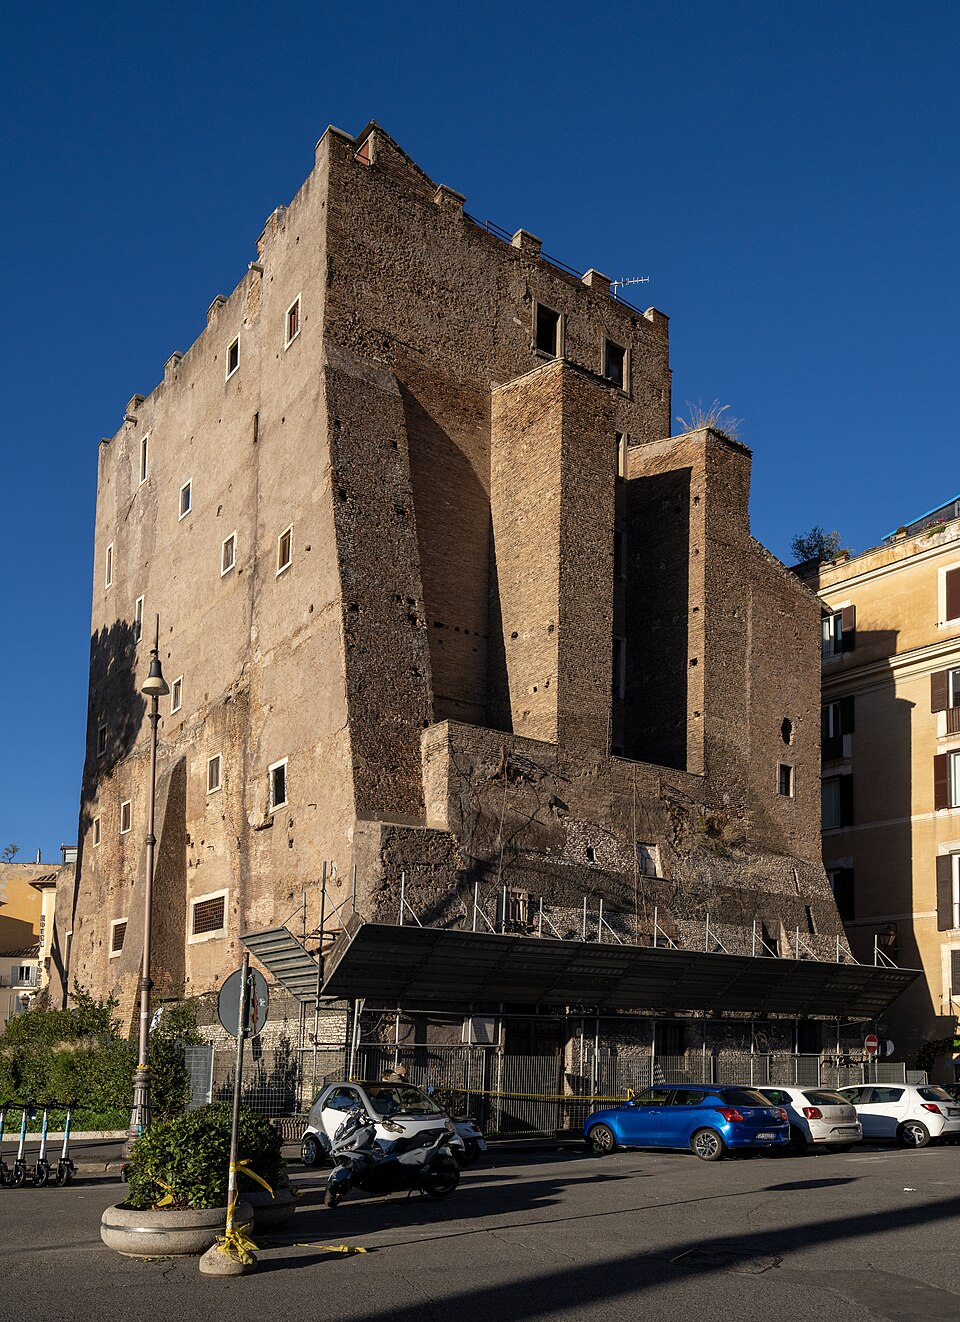
\includegraphics[width=0.3\textwidth]{graphics/torre_de_conti.jpg}
\caption{Torre de' Conti in its original state prior to the November 2025 collapse.}
\label{fig:torre_de_conti}
\end{figure}
\noindent